%% ============================================================
%%  CHAPTER 4 — SYSTEM OVERVIEW AND HARDWARE
%% ============================================================
\chapter{System Overview and Hardware}
\label{ch:hardware}

This chapter describes the physical realisation of the system: the
hardware that acquires the \acrshort{eeg} signal, runs the
classifier, and actuates the prosthetic hand, together with the way
these components are interconnected. Whereas Chapter~5 traces the
\emph{information} flow through the processing pipeline, this
chapter is concerned with the \emph{physical} platform on which that
pipeline runs --- the acquisition device, the compute host, the
microcontroller, the actuators, and the 3D-printed hand itself ---
and with the electrical interfaces that join them.

Section~\ref{sec:hw_overview} presents the end-to-end hardware
signal chain. Sections~\ref{sec:hw_acquisition}--\ref{sec:hw_hand}
describe each subsystem in turn: the acquisition hardware, the
compute hardware, the microcontroller and actuation electronics, and
the mechanical hand. Section~\ref{sec:hw_wiring} gives the complete
power and interconnection scheme, Section~\ref{sec:hw_bom}
summarises the bill of materials, and
Section~\ref{sec:hw_summary} closes the chapter.

%% ----------------------------------------------------------
\section{End-to-End Hardware Signal Chain}
\label{sec:hw_overview}
%% ----------------------------------------------------------

At the hardware level the system is a four-stage physical chain, as
shown in Figure~\ref{fig:hw_chain}. A scalp \acrshort{eeg} headset
acquires the raw signal and streams it to a Raspberry~Pi~5, which
runs the real-time inference pipeline of Chapter~12 and emits a
single discrete command label. That label is transmitted over a
\acrshort{uart} serial link to an ESP32 microcontroller, which
translates it into servo positions and drives the actuators of a
3D-printed InMoov prosthetic hand through a PCA9685 \acrshort{pwm}
controller. The same ESP32 also hosts the configuration web
application described in Chapter~11.

\begin{figure}[htbp]
\centering
\begin{tikzpicture}[
    node distance=0.9cm,
    hwbox/.style={rectangle, rounded corners=2pt, draw=black!70,
                  very thick, minimum width=3.0cm, minimum height=1.1cm,
                  align=center, font=\footnotesize, fill=red!10},
    lbl/.style={font=\scriptsize\itshape, align=center},
    arow/.style={-{Stealth[length=2.5mm]}, very thick},
]
\node[hwbox] (eeg) {EEG Headset\\\scriptsize scalp acquisition};
\node[hwbox, right=1.5cm of eeg] (pi) {Raspberry Pi 5\\\scriptsize classifier host};
\node[hwbox, right=1.5cm of pi] (esp) {ESP32\\\scriptsize hand controller};
\node[hwbox, right=1.5cm of esp] (hand) {InMoov Hand\\\scriptsize 6 servos};

\draw[arow] (eeg) -- node[lbl, above]{USB} (pi);
\draw[arow] (pi)  -- node[lbl, above]{UART\\115200 8N1} (esp);
\draw[arow] (esp) -- node[lbl, above]{PWM\\(PCA9685)} (hand);
\end{tikzpicture}
\caption{End-to-end hardware signal chain. A scalp EEG headset feeds
the Raspberry~Pi~5 classifier host over USB; the Pi sends discrete
command labels over UART to the ESP32, which drives the six servos of
the 3D-printed InMoov hand through a PCA9685 PWM controller.}
\label{fig:hw_chain}
\end{figure}

A deliberate design decision, discussed further in the limitations of
Chapter~13, is the separation of the \emph{classifier host}
(Raspberry~Pi~5) from the \emph{actuation controller} (ESP32). This
keeps the numerically intensive signal-processing and machine-learning
workload on a capable Linux computer, while delegating hard-real-time,
safety-critical motor control to a dedicated microcontroller that
never runs the classifier itself and therefore cannot be stalled by
it.

%% ----------------------------------------------------------
\section{EEG Acquisition Hardware}
\label{sec:hw_acquisition}
%% ----------------------------------------------------------

A distinction must be drawn between the hardware used to \emph{record}
the dataset and the hardware targeted for \emph{deployment}, because
they are not the same device --- a mismatch analysed as a limitation
in Chapter~\ref{ch:discussion}.

\paragraph{Data-collection device.}
The complete dataset of this project (Chapter~6) was recorded on a
19-channel research-grade \acrshort{eeg} system sampling at
\SI{200}{\hertz} and exporting to European Data Format
(\acrshort{edf}). Electrodes were placed according to the
International 10--20 system, with impedances kept below
\SI{20}{\kilo\ohm} at all sites. The frontal sites Fp1/Fp2 carry the
blink \acrshort{eog} commands and the temporal sites T3/T4 carry the
jaw \acrshort{emg} commands (Chapter~3). The recording amplifier and
its electrode leads are shown in Figure~\ref{fig:hw_eeg_device}.

\begin{figure}[htbp]
\centering
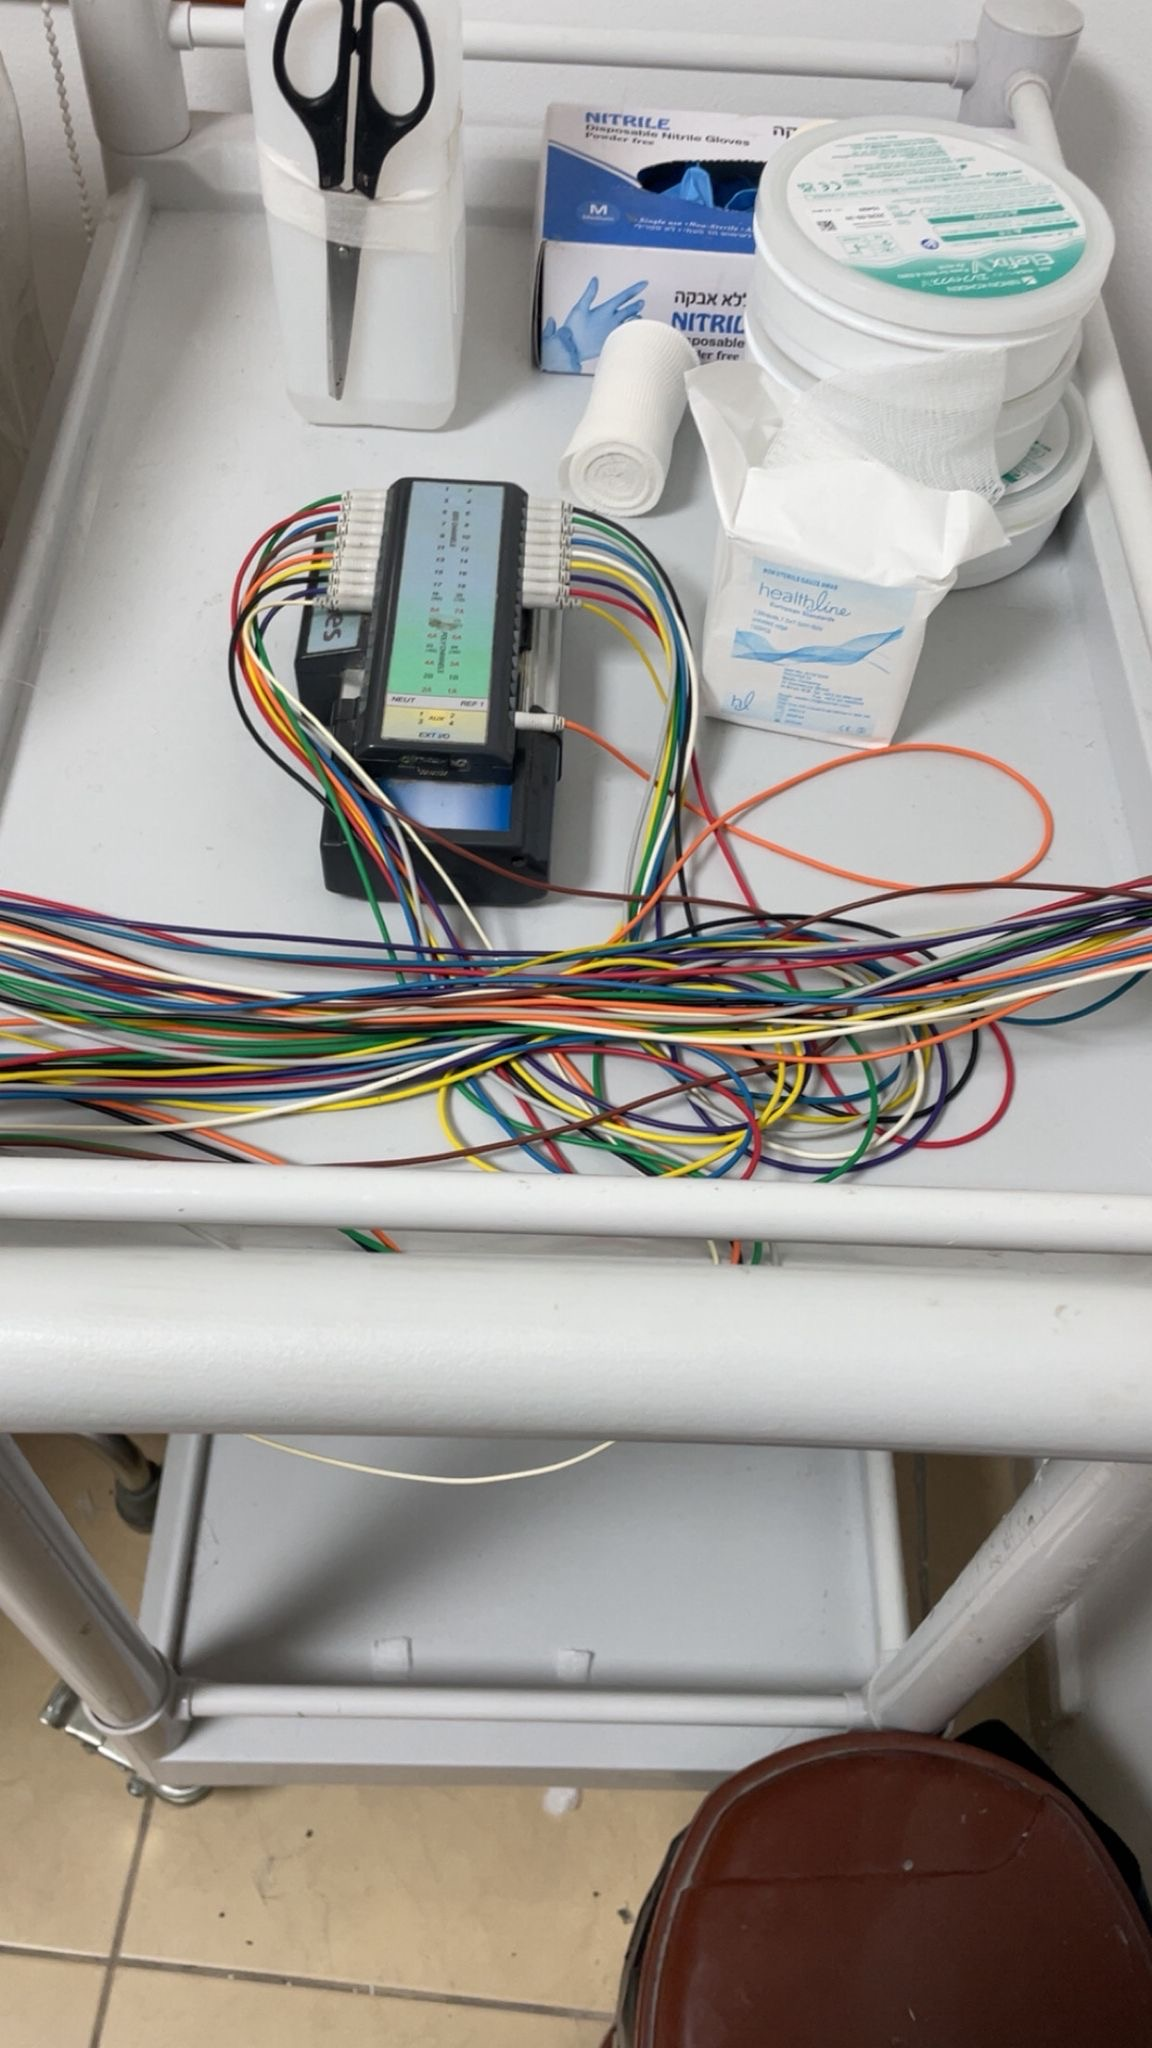
\includegraphics[width=0.6\textwidth]{Assets/eeg_device}
\caption{The 19-channel research-grade EEG amplifier (head-box) and
its colour-coded electrode leads used for data collection. Each lead
terminates at a scalp electrode placed per the International 10--20
system; the head-box digitises all channels and streams them to the
recording software.}
\label{fig:hw_eeg_device}
\end{figure}

\paragraph{Deployment target.}
The intended deployment headset is the \textbf{Emotiv EPOC~X}, a
14-channel consumer \acrshort{eeg} device connected to the
Raspberry~Pi~5 over its bundled USB receiver. The EPOC~X has a
different electrode layout and an on-device \SI{45}{\hertz} hardware
filter; channel correspondence with the research device is only
partial (T3/T4 map approximately to the Emotiv's T7/T8, and Fp1/Fp2
to AF3/AF4). No data has yet been collected on the target device to
validate transfer, which Chapter~13 identifies as the single largest
piece of outstanding validation.

Table~\ref{tab:hw_eeg} summarises both devices.

\begin{table}[htbp]
\centering
\caption{EEG acquisition hardware: data-collection vs.\ deployment.}
\label{tab:hw_eeg}
\begin{tabular}{@{}lll@{}}
\toprule
\textbf{Parameter} & \textbf{Data collection} & \textbf{Deployment target} \\
\midrule
Device        & 19-ch research-grade & Emotiv EPOC~X \\
Channels      & 19 (10--20)          & 14 \\
Sampling rate & \SI{200}{\hertz}     & on-device filtered \\
On-device filter & ---               & \SI{45}{\hertz} \\
Output        & EDF                  & USB stream \\
Host link     & recording software   & USB receiver $\to$ Pi 5 \\
\bottomrule
\end{tabular}
\end{table}

%% ----------------------------------------------------------
\section{Compute Hardware: The Classifier Host}
\label{sec:hw_compute}
%% ----------------------------------------------------------

The real-time inference pipeline (Chapter~12) is deployed on a
\textbf{Raspberry~Pi~5 (8\,GB)}. The Pi receives the live
\acrshort{eeg} stream over USB from the Emotiv receiver, executes the
full preprocessing, feature-extraction, and hybrid-classification
chain, applies the confidence and \acrshort{fsm} safety gates, and
emits the resulting command label over its hardware \acrshort{uart}
to the ESP32. The Pi is powered independently from the actuation
hardware (Section~\ref{sec:hw_wiring}); only a common ground is shared,
never the servo power rail.

%% ----------------------------------------------------------
\section{Microcontroller and Actuation Electronics}
\label{sec:hw_mcu}
%% ----------------------------------------------------------

The hand controller is an \textbf{ESP32-WROOM} mounted on a
Goouuu 38-pin (V4) expansion board whose DC jack accepts
\SIrange{6.5}{16}{\volt}. It receives command labels from the Pi over
\acrshort{uart} (GPIO16~=~RX, GPIO17~=~TX, common ground,
\SI{115200}{}~baud, 8N1; Chapter~11, Contract~A), maps each label to
a target pose, and drives the servos through a \textbf{PCA9685}
16-channel \acrshort{pwm} controller over the
\(\text{I}^2\text{C}\) bus (ESP32 GPIO21~=~SDA, GPIO22~=~SCL; PCA9685
at address \code{0x40}). The ESP32 additionally hosts the WiFi access
point and web application of Chapter~11. ESP32 was chosen over an
Arduino for its 16-bit \acrshort{pwm} resolution, integrated WiFi and
Bluetooth, and headroom to host the web application concurrently with
motor control.

\subsection{Servo Actuators}
\label{sec:hw_servos}

The hand is driven by \textbf{six MG996R servos} (operating range
\SIrange{4.8}{7.2}{\volt}), one per finger plus one for wrist
rotation, matching the six-element \code{servo\_angles} vector exposed
by the firmware (Chapter~11). Each servo is set to its start angle
before mounting. Table~\ref{tab:hw_servos} gives the channel
assignment.

\begin{table}[htbp]
\centering
\caption{Actuation channel assignment (six MG996R servos on the PCA9685).}
\label{tab:hw_servos}
\begin{tabular}{@{}clc@{}}
\toprule
\textbf{Channel} & \textbf{Joint} & \textbf{Start angle} \\
\midrule
CH0 & Thumb  & \ang{150} \\
CH1 & Index  & \ang{150} \\
CH2 & Middle & \ang{150} \\
CH3 & Ring   & \ang{150} \\
CH4 & Pinky  & \ang{150} \\
CH5 & Wrist  & \ang{90} (centre) \\
\bottomrule
\end{tabular}
\end{table}

%% ----------------------------------------------------------
\section{The Prosthetic Hand: Mechanical Design}
\label{sec:hw_hand}
%% ----------------------------------------------------------

The mechanical hand is based on the open-source \textbf{InMoov}
design~\cite{langevin2026inmoov}, combining three InMoov component generations:
the newest \emph{i2} right hand (fingers, palm, covers), the classic
\emph{robpart} forearm shell, and a \emph{RotaWrist} module that
physically bridges the two --- the i2 hand bolts to RotaWrist3 above
(M8 joint) while RotaWrist1 is epoxied to the forearm shell below.

The structural parts are 3D-printed in \textbf{PLA+} (white), while
the \textbf{fingertips are printed in TPU} for a compliant, higher-grip
contact surface. Printing used a \SI{0.4}{\milli\meter} nozzle with
\SI{1.75}{\milli\meter} filament at a \SI{0.25}{\milli\meter} layer
height (reduced to \SI{0.15}{\milli\meter} for gears and pulleys) and
30\% infill (50\% for gears and pulleys), consuming roughly
\SI{850}{\gram} of filament in total.

Actuation is tendon-driven: braided fishing line
(\SI{0.8}{\milli\meter}, 200\,lb) runs from a servo-horn pulley in the
forearm servo bed, through a dedicated \acrshort{ptfe} Bowden tube
(ID \SI{1.5}{\milli\meter} / OD \SI{2.5}{\milli\meter}, one per finger)
that eliminates friction against the printed plastic, to each
fingertip; extension springs return each finger when the tendon
relaxes. Five servos sit in the forearm servo bed for the fingers, and
the sixth drives wrist rotation through the RotaWrist gear.

Figure~\ref{fig:hw_hand_photo} shows the assembled hand.

\begin{figure}[htbp]
\centering
% \includegraphics[width=0.6\textwidth]{Assets/prosthetic_hand.jpg}
\TODO{Insert a photograph of the assembled 3D-printed InMoov hand ---
save it as e.g.\ Assets/prosthetic\_hand.jpg and uncomment the
\textbackslash includegraphics line above. A close-up of the forearm
servo bed and wiring would also strengthen this section.}
\caption{The assembled 3D-printed InMoov (i2 hand + classic forearm +
RotaWrist) prosthetic hand used in this project.}
\label{fig:hw_hand_photo}
\end{figure}

%% ----------------------------------------------------------
\section{Power Distribution and Interconnection}
\label{sec:hw_wiring}
%% ----------------------------------------------------------

Power originates from a \textbf{\SI{12}{\volt}, \SI{5}{\ampere}
mains SMPS} and splits two ways, as shown in
Figure~\ref{fig:hw_wiring}. One branch feeds \SI{12}{\volt} directly
to the ESP32 expansion board's DC jack (rated
\SIrange{6.5}{16}{\volt}; its onboard regulator derives the
\SI{5}{\volt} logic rail internally). The other branch passes through
an \textbf{XL4015 buck converter} stepped down to \textbf{exactly
\SI{6}{\volt}} --- set and verified on the converter's LED display
\emph{before} any servo is connected --- which supplies the PCA9685
\(V\!+\) servo rail. A \textbf{\SI{470}{\micro\farad} capacitor}
across the \SI{6}{\volt} rail at the PCA9685 absorbs the inrush when
several servos move at once, preventing brownout resets of the
controller. The \SI{12}{\volt} rail never touches the servos or the
PCA9685 \(V\!+\); all grounds are tied common. The Raspberry~Pi~5 is
powered separately from its own USB-C supply, sharing only ground.

\begin{figure}[htbp]
\centering
\begin{tikzpicture}[
    node distance=0.8cm and 1.2cm,
    comp/.style={rectangle, rounded corners=2pt, draw=black!70,
                 very thick, minimum width=2.7cm, minimum height=0.95cm,
                 align=center, font=\scriptsize, fill=blue!8},
    pwr/.style={comp, fill=orange!15},
    srv/.style={comp, fill=green!12, minimum width=2.4cm, minimum height=0.7cm},
    lbl/.style={font=\tiny, align=center},
    sig/.style={-{Stealth[length=2mm]}, thick},
    hi/.style={-{Stealth[length=2mm]}, very thick, red!70!black},
    lo/.style={-{Stealth[length=2mm]}, very thick, orange!80!black},
]
% Power spine
\node[pwr] (mains) {220V mains};
\node[pwr, right=of mains] (smps) {12V SMPS\\\scriptsize 12V 5A};
\node[comp, right=1.6cm of smps] (esp) {ESP32\\\scriptsize + expansion};
\node[pwr, below=1.0cm of smps] (buck) {XL4015 buck\\\scriptsize set to 6.0V};
\node[comp, right=1.6cm of buck] (pca) {PCA9685\\\scriptsize V+ 6V, VCC 5V};
\node[comp, fill=blue!8, above=1.0cm of esp] (pi) {Raspberry Pi 5};

% Servo stack
\node[srv, right=1.5cm of pca, yshift=1.4cm]  (s0) {CH0 Thumb};
\node[srv, below=0.15cm of s0] (s1) {CH1 Index};
\node[srv, below=0.15cm of s1] (s2) {CH2 Middle};
\node[srv, below=0.15cm of s2] (s3) {CH3 Ring};
\node[srv, below=0.15cm of s3] (s4) {CH4 Pinky};
\node[srv, below=0.15cm of s4] (s5) {CH5 Wrist};

% Power flow
\draw[sig] (mains) -- (smps);
\draw[hi] (smps) -- node[lbl,above]{12V direct} (esp);
\draw[hi] (smps) -- node[lbl,left]{12V} (buck);
\draw[lo] (buck) -- node[lbl,above]{6V} (pca);

% Signal
\draw[sig] (pi) -- node[lbl,left]{UART} (esp);
\draw[sig, dashed] (esp) -- node[lbl,right]{5V + I\textsuperscript{2}C} (pca);

% PWM fan-out
\foreach \s in {s0,s1,s2,s3,s4,s5}{ \draw[lo] (pca.east) -- (\s.west); }
\node[lbl] at ($(pca.east)!0.5!(s3.west)+(0,0.15)$) {PWM};
\end{tikzpicture}
\caption{Power distribution and interconnection. The 12\,V, 5\,A SMPS
splits: 12\,V directly to the ESP32 expansion board, and 12\,V through
an XL4015 buck set to 6\,V that supplies the PCA9685 servo rail (with
a 470\,\textmu F smoothing capacitor). The ESP32 drives the PCA9685
over I\textsuperscript{2}C, which fans out PWM to the six MG996R
servos; the Pi 5 links to the ESP32 by UART and is powered separately.
All grounds are common.}
\label{fig:hw_wiring}
\end{figure}

The complete point-to-point wiring, including the
\(\text{I}^2\text{C}\) jumper assignment (ESP32 GPIO21/22 to PCA9685
SDA/SCL, \SI{5}{\volt}, GND) and the servo channel orientation
(brown\,$\to$\,GND, red\,$\to$\,\(V\!+\), orange\,$\to$\,signal), is
carried out in the strict phase order that guarantees the buck
converter is set to \SI{6}{\volt} before any servo or the PCA9685
\(V\!+\) rail is energised.

%% ----------------------------------------------------------
\section{Bill of Materials}
\label{sec:hw_bom}
%% ----------------------------------------------------------

Table~\ref{tab:hw_bom} lists the principal hardware components.

\begin{table}[htbp]
\centering
\caption{Principal hardware bill of materials.}
\label{tab:hw_bom}
\begin{tabular}{@{}llc@{}}
\toprule
\textbf{Component} & \textbf{Specification} & \textbf{Qty} \\
\midrule
EEG headset (deployment) & Emotiv EPOC~X, 14-ch, USB      & 1 \\
Compute host             & Raspberry Pi 5, 8\,GB          & 1 \\
Microcontroller          & ESP32-WROOM + Goouuu 38P/V4    & 1 \\
PWM driver               & PCA9685, 16-ch, $\text{I}^2\text{C}$ & 1 \\
Servos                   & MG996R, \SIrange{4.8}{7.2}{\volt} & 6 \\
Mains supply             & 12\,V / 5\,A SMPS              & 1 \\
Buck converter           & XL4015 (12\,V\,$\to$\,6\,V, LED) & 1 \\
Smoothing capacitor      & \SI{470}{\micro\farad}         & 1 \\
Prosthetic hand          & InMoov i2 + forearm, PLA+ / TPU tips & 1 \\
Tendons                  & braided line + PTFE Bowden tube & set \\
\bottomrule
\end{tabular}
\end{table}

%% ----------------------------------------------------------
\section{Chapter Summary}
\label{sec:hw_summary}
%% ----------------------------------------------------------

This chapter described the physical platform of the system. The
dataset was recorded on a 19-channel research-grade \acrshort{eeg}
device, while the deployment target is the 14-channel Emotiv EPOC~X
connected over USB to a Raspberry~Pi~5 (8\,GB) classifier host. The Pi
drives an ESP32-WROOM hand controller over \acrshort{uart}; the ESP32
actuates six MG996R servos of a 3D-printed InMoov hand through a
PCA9685 \acrshort{pwm} controller, and hosts the configuration web
application of Chapter~11. A 12\,V / 5\,A SMPS powers the system, with
a dedicated XL4015 buck rail at 6\,V for the servos and a common
ground throughout. The deliberate separation of classifier host and
actuation controller localises hard-real-time, safety-critical motor
control on a dedicated microcontroller. With the physical platform
established, Chapter~5 now gives the end-to-end methodology that runs
on top of it.